
%(BEGIN_QUESTION)
% Copyright 2015, Tony R. Kuphaldt, released under the Creative Commons Attribution License (v 1.0)
% This means you may do almost anything with this work of mine, so long as you give me proper credit

Sketch a phasor diagram for this transformer bank's output voltages, and determine their phase rotation:

$$\includegraphics[width=15.5cm]{i00835x01.eps}$$

\vfil 

\underbar{file i00835}
\eject
%(END_QUESTION)





%(BEGIN_ANSWER)

This is a graded question -- no answers or hints given!

%(END_ANSWER)





%(BEGIN_NOTES)

First, a phasor diagram showing the primary winding voltages:

$$\includegraphics[width=15.5cm]{i00835x02.eps}$$

Each transformer steps its primary voltage down by a factor of 20 (i.e. 398.4 volts at each secondary winding).  Phase angles, of course, are maintained from primary winding to secondary winding, measured from terminal 1 to terminal 2.  This means:

$$V_{XZ} = 398.4 \hbox{ V} \angle 15^o$$  

$$V_{YX} = 398.4 \hbox{ V} \angle -105^o$$  

$$V_{ZY} = 398.4 \hbox{ V} \angle 135^o$$  

\vskip 10pt

Sketching these three phasors on a diagram of their own.  Note how phasor XY has the same orientation (angle) as phasor A from the previous phasor diagram, and how phasor ZY matches the angle of phasor C, and how phasor YX matches the angle of phasor B:

$$\includegraphics[width=15.5cm]{i00835x03.eps}$$

Labeling each vertex of the phasor Delta, we see the rotation XYZ for this transformer bank's output.  Output phase voltage $V_X$ happens to have an angle of 45$^{o}$, leading $V_A$ by 30 degrees.

%INDEX% Electronics review: 3-phase electrical power 
%INDEX% Electronics review, phasor expressions of circuit quantities

%(END_NOTES)


